\documentclass[a4paper, 11pt]{article}
\usepackage{amsmath}
\usepackage{amssymb}
\usepackage{graphicx}
\usepackage{indentfirst}

\author{One \& Two}
\title{Surface minimale en dimension finie}

\begin{document}
\maketitle
\newpage

\section{Probl\`eme de surface minimale en dimension infinie}
Soit $\Omega$ un sous-ensemble born\'e de $\mathbb{R}^2$ \`a fronti\`ere
 lipschitzienne. Soit $g\in\mathcal{C}^0(\partial\Omega)$. Le probl\`eme de
 surface minimale est le suivant:
\begin{equation}
\begin{cases}
\min\limits_{u\in H^1(\Omega)}\int\limits_\Omega\sqrt{1+|\nabla u|^2}\,
\mathrm{d}\lambda \\
u_{|\partial\Omega}=g
\end{cases}
\end{equation}
On pose:
$$
\forall x\in\Omega, \forall u\in H^1(\Omega), L(x, u(x), \nabla u(x))=
\sqrt{1+|\nabla u(x)|^2}
$$
Et on note:
$$
\forall u\in H^1(\Omega), J(u)=\int\limits_\Omega L(x, u(x), \nabla u(x))
\,\mathrm{d}\lambda
$$
Le probl\`eme de surface minimale est le suivant:
\begin{equation}
\begin{cases}
\min\limits_{u\in H^1(\Omega)}J(u) \\
u_{|\partial\Omega}=g
\end{cases}
\end{equation}
Si la fonctionnelle $J$ admet un minimum $u$ alors pour tous $v\in H^1(\Omega)$,
 la diff\'erentielle de $J$ verifie:
\begin{align*}
\langle dJ(u), v\rangle &= \int\limits_\Omega\langle dL(x, u(x), \nabla u(x)),
v(x)\rangle\,\mathrm{d}\lambda \\
&= \int\limits_\Omega\frac{\langle \nabla u(x), \nabla v(x)\rangle}{L(x, u(x),
 \nabla u(x))}\,\mathrm{d}\lambda
\end{align*}
Et:
$$
\langle dJ(u), v\rangle = 0
$$
\newpage
\section{Probl\`eme de surface minimale en dimension finie}
TODO: formules
\subsection{Questions}
Q1) On a que $u^0$ ne change pas \\

Q3) Voir code: test3.cpp \\

Q4) Pour la cat\'eno\"ide, on a bien voici les valeurs: \\

$$
\begin{array}{|c|c|c|}
\hline
\text{It\'eration} & \text{It\'eration du gradient} & \text{Erreur cons\'ecutive}
 \\
\hline
0 & 87 & 2.67709 \\
1 & 74 & 1.02045 \\
2 & 70 & 0.562683 \\
3 & 66 & 0.331348 \\
4 & 64 & 0.195968 \\
5 & 62 & 0.114703 \\
6 & 60 & 0.0663983 \\
7 & 59 & 0.0381426 \\
8 & 57 & 0.021824 \\
9 & 55 & 0.0124709 \\
10 & 53 & 0.00712846 \\
30 & 15 & 1.17025e^{-07} \\
31 & 13 & 6.76511e^{-08} \\
32 & 12 & 3.91262e^{-08} \\
33 & 11 & 2.262e^{-08} \\
34 & 10 & 1.30502e^{-08} \\
35 & 10 & 7.57321e^{-09} \\
36 & 6 & 3.63576e^{-09} \\
37 & 6 & 2.58286e^{-09} \\
38 & 2 & 8.17945e^{-10} \\
39 & 2 & 6.0615e^{-10} \\
40 & 0 & 0 \\
\hline
\end{array}
$$

\begin{figure}[h!]
  \centering
  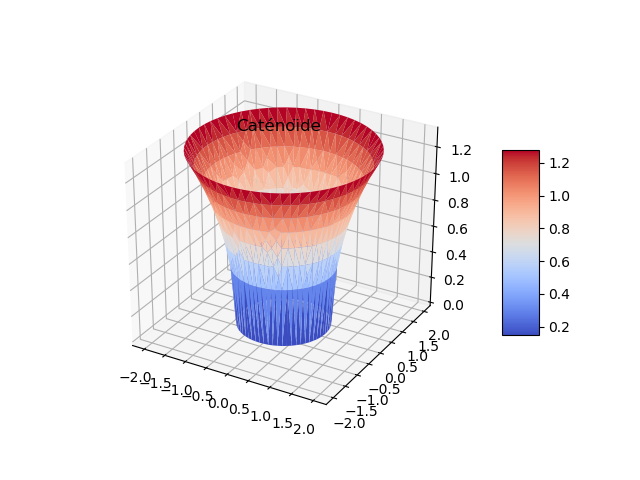
\includegraphics[width=\linewidth]{catenoide.png}
  \caption{La cat\'eno\"ide.}
  \label{fig:catenoide}
\end{figure}

\newpage

Q5) Voir code: test5.cpp . Voici les valeurs: \\
$$
\begin{array}{|c|c|c|}
\hline
\text{It\'eration} & \text{It\'eration du gradient} & \text{Erreur cons\'ecutive}
 \\
\hline
0 & 55 & 5.54098 \\
1 & 51 & 1.37066 \\
2 & 49 & 0.37741 \\
3 & 49 & 0.0963363 \\
4 & 48 & 0.0237973 \\
5 & 46 & 0.00588999 \\
6 & 44 & 0.00148339 \\
7 & 42 & 0.000383801 \\
8 & 40 & 0.000103052 \\
9 & 37 & 2.90305e^{-05} \\
10 & 35 & 8.64873e^{-06} \\
11 & 33 & 2.72588e^{-06} \\
12 & 31 & 9.01889e^{-07} \\
13 & 27 & 3.09612e^{-07} \\
14 & 22 & 1.09021e^{-07} \\
15 & 18 & 3.8991e^{-08} \\
16 & 8 & 1.39172e^{-08} \\
17 & 4 & 5.08228e^{-09} \\
18 & 3 & 1.90381e^{-09} \\
19 & 3 & 8.07361e^{-10} \\
20 & 1 & 2.32879e^{-10} \\
21 & 0 & 0 \\
\hline
\end{array}
$$

\begin{figure}[h!]
  \centering
  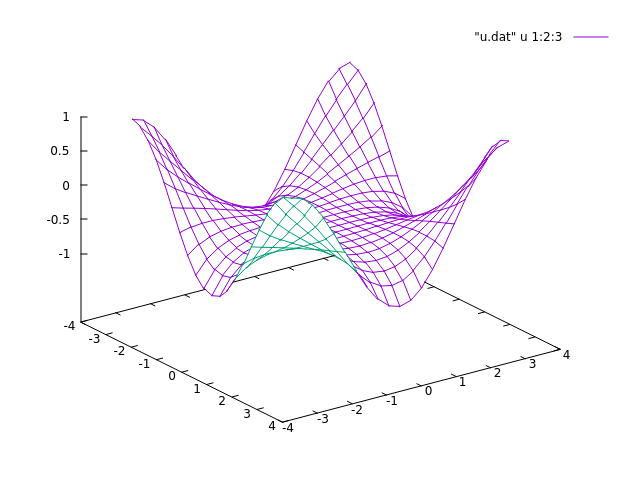
\includegraphics[width=\linewidth]{cos_cos.png}
  \caption{$(x, y)\mapsto\cos(x)\cos(y)$.}
  \label{fig:cos_cos}
\end{figure}

\newpage

Q6) Quelques cas
\end{document}

